
\documentclass[../../../all/physics-standard_questions_all.tex]{subfiles}

\graphicspath{{../../../../figures/}}

\begin{document}

\setlength{\abovedisplayskip}{2mm}
\setlength{\belowdisplayskip}{1mm}

抵抗A（抵抗値10\,$\Omega$）と抵抗B（抵抗値40\,$\Omega$），
電池（起電力10\,V，内部抵抗無視），および図\ref{q_circuit-extent_02_01}に示すような電流・電圧特性をもつ豆電球を用意する．

\begin{enumerate}

    \item 豆電球を電池に接続する．豆電球を流れる電流の大きさを求めよ．

    \item 同じ豆電球を2つ直列につなぎ，電池に接続する．豆電球を流れる電流の大きさを求めよ．

    \item 図\ref{q_circuit-extent_02_02}のように抵抗Aと豆電球を直列につなぎ，電池に接続する．
        豆電球を流れる電流の大きさを求めよ．

    \item 図\ref{q_circuit-extent_02_03}のように抵抗Bを豆電球に並列につなぎ，これらに抵抗Aを直列につないで，
        電池に接続する．豆電球を流れる電流の大きさを求めよ．

\end{enumerate}

\setcounter{figure}{0}

\vspace{0.2\baselineskip}
{\centering
    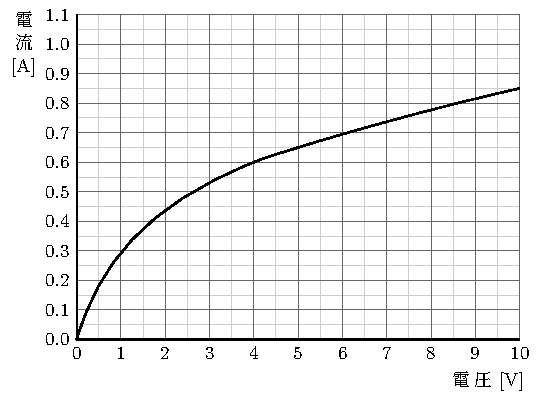
\includegraphics{q_circuit-extent_02_01/physics-standard_questions_circuit-extent_02_01_tikz.pdf}
    \captionof{figure}{} \label{q_circuit-extent_02_01}
\par}

\vspace{0.5\baselineskip}

{\centering
    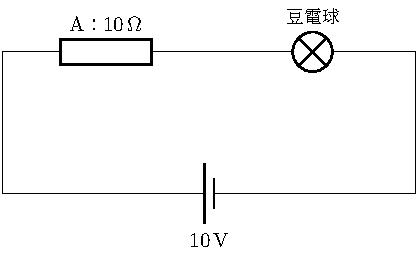
\includegraphics{q_circuit-extent_02_02/physics-standard_questions_circuit-extent_02_02_tikz.pdf}
    \captionof{figure}{} \label{q_circuit-extent_02_02}
    \par}

\vspace{0.5\baselineskip}

{\centering
    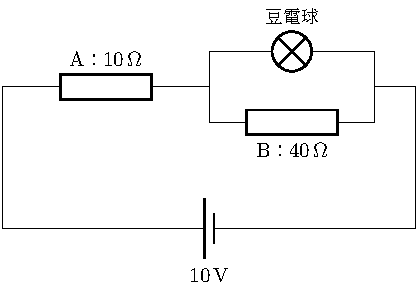
\includegraphics{q_circuit-extent_02_03/physics-standard_questions_circuit-extent_02_03_tikz.pdf}
    \captionof{figure}{} \label{q_circuit-extent_02_03}
\par}

\vspace{0.2\baselineskip}

\end{document}
